%% ----------------------------------------------------------------
%% Evaluation.tex
%% ---------------------------------------------------------------- 
\chapter{Evaluation} \label{Chapter:Evaluation}

\section{Localised Design}

The test set is fed into the trained localised model to give a general sense of how well did the model predict. 
By collecting all of the predictions together, predictions and the actual target values are plotted in \fref{Figure:eva_all}.
The graph shows a good prediction in long-term trends of the travel time, yet there are some biases. 

In the actual values, there are large fluctuations of values, these rapid changes have not been well predicted by the model. 
The values predicted are rather conservative, focusing more on the long-term trends, and tend to ignore the high-frequency fluctuations. 

\begin{figure}[!htb]
    \centering
    \subcaptionbox{Half of the test set}{
        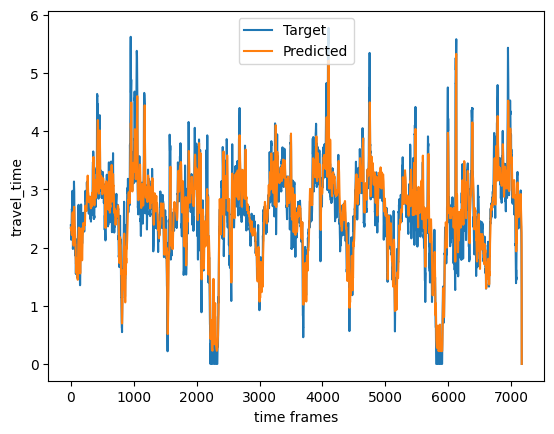
\includegraphics[width=0.48\linewidth]{eva_whole}
        \label{Figure:eva_whole}
    }
    \subcaptionbox{One day}{
        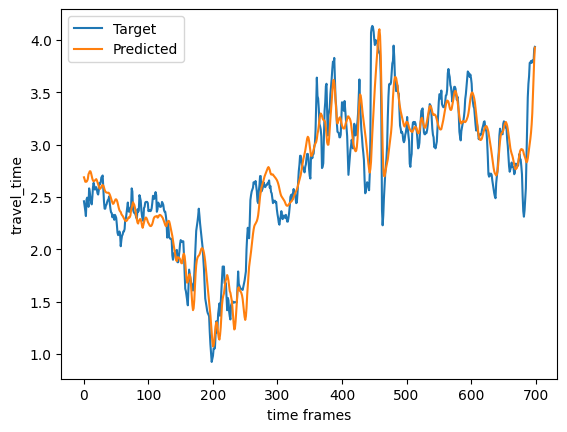
\includegraphics[width=0.48\linewidth]{eva_local}
        \label{Figure:eva_local}
    }
    \caption{Predictions from the localised design joined together compared with the actual values}
    \label{Figure:eva_all}
\end{figure}

Due to the fact that the model only predicts the next 15 minutes in advance, such a graph does not tell much about the situation to use the model.
Instead, each predictions are plotted individually with the true values. Some prepresentative examples are shown in \fref{Figure:predict}.
The first 30 data points are the inputs that feed into the model, after that comes the predictions. 
Generally, the predictions show a smooth curve that has a starting point very close to the last time frame in the inputs. 
The first few data points predicted are more accurate compared to the later ones.

\fref{Figure:fault} is an example of a prediction that has a trend that completely does not agree with the actual values. 
This is a fault prediction that happens more frequently when there is a significant increase in travel time in a short period. 
This may be due to unaccounted-for external factors and unexpected events, such as accidents. This does affect the applications of the model, like a navigation application. 
Predictions like this will affect the decision made on selecting roads and the expected time taken calculated. 

\begin{figure}[!htb]
    \centering
    \subfloat[Fault prediction\label{Figure:fault}]{
        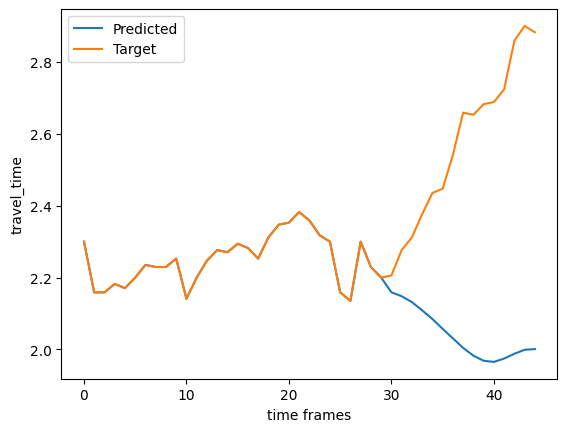
\includegraphics[width=0.48\linewidth]{eva_1}
    }
    \subfloat[Correct trends with conservative values\label{Figure:trends}]
    {
        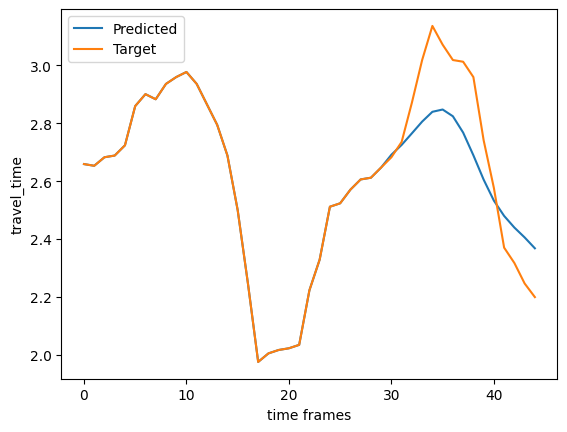
\includegraphics[width=0.48\linewidth]{eva_2}
    }
    
    \subfloat[Correct trends and values\label{Figure:correct}]{
        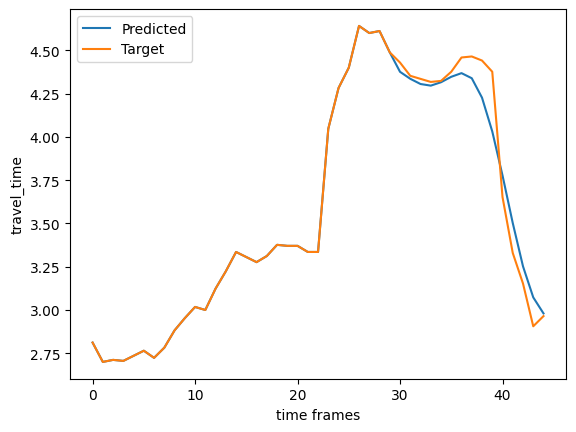
\includegraphics[width=0.48\linewidth]{eva_3}
    }
    \subfloat[Sudden change in values\label{Figure:change}]
    {
        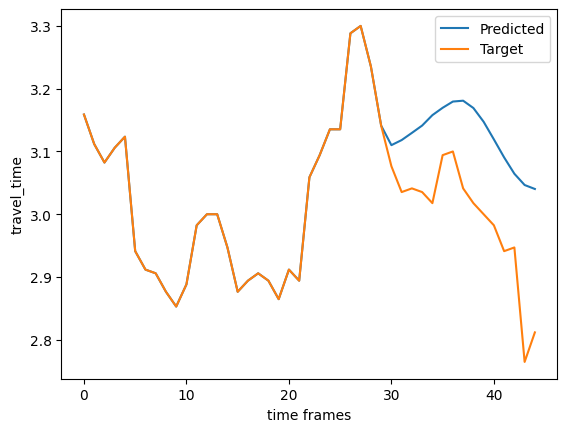
\includegraphics[width=0.48\linewidth]{eva_4}
    }
    \caption{Representative predictions in the test set}
    \label{Figure:predict}
\end{figure}

The prediction of \fref{Figure:trends} predicts the trend correctly but with a lower amplitude. 
The LSTM model generally has the nature of smoothness, which predicts noises and sudden changes relatively stably. 
It implies that the model mainly learns the general trends and cyclical changes in the data, but fails to fully capture the sudden changes in the real values. 
Also, the model may filter out some of the fluctuations as noise or outliers, which also makes the predicted values relatively smooth. 

\fref{Figure:change} have a similar condition when there is a sudden change. This time the change is given in the input sequence. 
The prediction shows a correct trend but the values are closer to the value of the last of the input sequence. 
As long as the the trend is correctly predicted, it will be fine to use since it will not affect much on decision makings. 

\fref{Figure:correct} gives an accurate prediction that it correctly predicts the trend and values. 
This is an ideal situation. These accurate predictions happen more when there is a drop in travel time. 
This may be because the characteristics of the drop are clearer than a rise in travel time in the dataset. The model successfully captures the pattern and makes good predictions. 

\section{Globalised Design}

The predictions of a single link using the GCN-LSTM model are worse compared to the localised design. 
The benefit of it is that it predicts a total of 132 links together at once. 
\fref{Figure:eva_global} shows the one-day predictions of one of the links compared with the targets.

\begin{figure}[!htb]
    \centering
    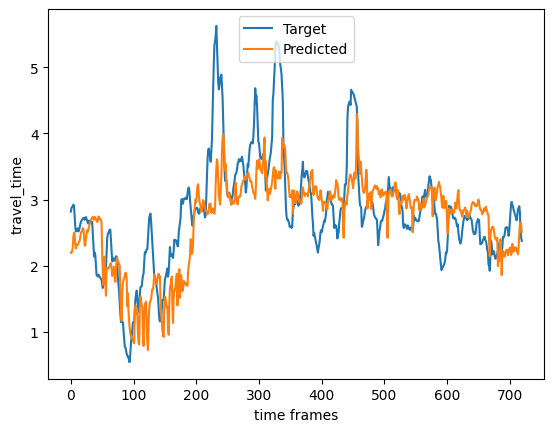
\includegraphics[width=11cm]{eva_global}
    \caption{Predictions of one link from the GCN-LSTM model joined together compared with the actual values}
    \label{Figure:eva_global}
\end{figure}

The predictions are still not far from the actual values but are a lot more off than the localised ones. 
The predictions seem lagging behind, it needs some time to adapt the jumps of the actual values. This shows that the model does not have a good ability to predict the sudden changes. 
The LSTM layers are not able to handle all links at the same time to give the same level of accuracy as for only one link.

The current performance of the GCN-LSTM model with inputs used is not ideal to be used in applications that require accurate predictions in a short period of time.
There are many more parameters and selections that could be made to optimise the performance of the model which have not been covered in the project. 
